\documentclass[11pt,twocolumn,oneside,openany,headings=optiontotoc,11pt,numbers=noenddot]{article}

\usepackage[a4paper]{geometry}
\usepackage[utf8]{inputenc}
\usepackage[T1]{fontenc}
\usepackage{lmodern}
\usepackage[ngerman]{babel}
\usepackage{ngerman}

\usepackage[onehalfspacing]{setspace}

\usepackage{fancyhdr}
\usepackage{fancybox}

\usepackage{rotating}
\usepackage{varwidth}

%Struktogramme
\usepackage[german,curves]{struktex}

\usepackage{pdflscape}
\usepackage{changepage}
\usepackage{graphicx}
\usepackage[bottom]{footmisc}
\usepackage{transparent}
\usepackage{graphbox}
\graphicspath{
	{Pics/PDFs/}
	{Pics/JPGs/}
	{Pics/PNGs/}
}
\usepackage{caption}
\usepackage{wrapfig}
\usepackage{marginnote}
\usepackage{tabularx}
\usepackage{dashrule}
\usepackage{soulutf8}
\usepackage{hhline}
%arydshln suppresses vertical lines in table
%\usepackage{arydshln}
\usepackage{multirow}
\usepackage{enumerate}
\usepackage[hidelinks]{hyperref}
\usepackage{listings}

\usepackage[table]{xcolor}
\usepackage{array}
\usepackage{enumitem,amssymb,amsmath}
\usepackage{interval}
\usepackage{cancel}
\usepackage{stmaryrd}
\usepackage{wasysym}
\usepackage{polynom}
\usepackage{diagbox}
\usepackage{dashrule}
\usepackage{framed}
\usepackage{mdframed}
\usepackage{karnaugh-map}
\usepackage{pdfpages}

\usepackage{blindtext}

\usepackage{eso-pic}

\usepackage{amssymb}
\usepackage{eurosym}

\usepackage[pages=some]{background}
\pagestyle{headings}
\renewcommand{\headrulewidth}{0.2pt}
\renewcommand{\footrulewidth}{0.2pt}
\newcommand*{\underdownarrow}[2]{\ensuremath{\underset{\overset{\Big\downarrow}{#2}}{#1}}}
\setlength{\fboxsep}{5pt}
\newcommand{\explainBelow}[3]{\underbrace{#1}_{\parbox{\widthof{#3}}{\footnotesize\raggedright #2}}}
\newcommand{\explainAbove}[3]{\overbrace{#1}^{\parbox{\widthof{#3}}{\footnotesize\raggedright #2}}}
\newcommand\footnoteref[1]{\protected@xdef\@thefnmark{\ref{#1}}\@footnotemark}


% Codestyle defined
\definecolor{codegreen}{rgb}{0,0.6,0}
\definecolor{codegray}{rgb}{0.5,0.5,0.5}
\definecolor{codepurple}{rgb}{0.58,0,0.82}
\definecolor{backcolour}{rgb}{0.95,0.95,0.92}
\definecolor{deepgreen}{rgb}{0,0.5,0}
\definecolor{darkblue}{rgb}{0,0,0.65}
\definecolor{mauve}{rgb}{0.40, 0.19,0.28}
\colorlet{exceptioncolour}{yellow!50!red}
\colorlet{commandcolour}{blue!60!black}
\colorlet{numpycolour}{blue!60!green}
\colorlet{specmethodcolour}{violet}

%Neue Spaltendefinition
\newcolumntype{L}[1]{>{\raggedright\let\newline\\\arraybackslash\hspace{0pt}}m{#1}}
\newcolumntype{M}{>{\centering\arraybackslash}X}
\newcommand{\cmnt}[1]{\ignorespaces}
%Textausrichtung ändern
\newcommand\tabrotate[1]{\rotatebox{90}{\raggedright#1\hspace{\tabcolsep}}}

%Intervall-Konfig
\intervalconfig {
	soft open fences
}

%Bash
\lstdefinestyle{BashInputStyle}{
	language=bash,
	basicstyle=\small\sffamily,
	backgroundcolor=\color{backcolour},
	columns=fullflexible,
	backgroundcolor=\color{backcolour},
	breaklines=true,
}
%Java
\lstdefinestyle{JavaInputStyle}{
	language=Java,
	backgroundcolor=\color{backcolour},
	aboveskip=1mm,
	belowskip=1mm,
	showstringspaces=false,
	columns=flexible,
	basicstyle={\footnotesize\ttfamily},
	numberstyle={\tiny},
	numbers=none,
	keywordstyle=\color{purple},,
	commentstyle=\color{deepgreen},
	stringstyle=\color{blue},
	emph={out},
	emphstyle=\color{darkblue},
	emph={[2]rand},
	emphstyle=[2]\color{specmethodcolour},
	breaklines=true,
	breakatwhitespace=true,
	tabsize=2,
}
%Python
\lstdefinestyle{PythonInputStyle}{
	language=Python,
	alsoletter={1234567890},
	aboveskip=1ex,
	basicstyle=\footnotesize,
	breaklines=true,
	breakatwhitespace= true,
	backgroundcolor=\color{backcolour},
	commentstyle=\color{red},
	otherkeywords={\ , \}, \{, \&,\|},
	emph={and,break,class,continue,def,yield,del,elif,else,%
		except,exec,finally,for,from,global,if,import,in,%
		lambda,not,or,pass,print,raise,return,try,while,assert},
	emphstyle=\color{exceptioncolour},
	emph={[2]True,False,None,min},
	emphstyle=[2]\color{specmethodcolour},
	emph={[3]object,type,isinstance,copy,deepcopy,zip,enumerate,reversed,list,len,dict,tuple,xrange,append,execfile,real,imag,reduce,str,repr},
	emphstyle=[3]\color{commandcolour},
	emph={[4]ode, fsolve, sqrt, exp, sin, cos, arccos, pi,  array, norm, solve, dot, arange, , isscalar, max, sum, flatten, shape, reshape, find, any, all, abs, plot, linspace, legend, quad, polyval,polyfit, hstack, concatenate,vstack,column_stack,empty,zeros,ones,rand,vander,grid,pcolor,eig,eigs,eigvals,svd,qr,tan,det,logspace,roll,mean,cumsum,cumprod,diff,vectorize,lstsq,cla,eye,xlabel,ylabel,squeeze},
	emphstyle=[4]\color{numpycolour},
	emph={[5]__init__,__add__,__mul__,__div__,__sub__,__call__,__getitem__,__setitem__,__eq__,__ne__,__nonzero__,__rmul__,__radd__,__repr__,__str__,__get__,__truediv__,__pow__,__name__,__future__,__all__},
	emphstyle=[5]\color{specmethodcolour},
	emph={[6]assert,range,yield},
	emphstyle=[6]\color{specmethodcolour}\bfseries,
	emph={[7]Exception,NameError,IndexError,SyntaxError,TypeError,ValueError,OverflowError,ZeroDivisionError,KeyboardInterrupt},
	emphstyle=[7]\color{specmethodcolour}\bfseries,
	emph={[8]taster,send,sendMail,capture,check,noMsg,go,move,switch,humTem,ventilate,buzz},
	emphstyle=[8]\color{blue},
	keywordstyle=\color{blue}\bfseries,
	rulecolor=\color{black!40},
	showstringspaces=false,
	stringstyle=\color{deepgreen}
}

\lstset{literate=%
	{Ö}{{\"O}}1
	{Ä}{{\"A}}1
	{Ü}{{\"U}}1
	{ß}{{\ss}}1
	{ü}{{\"u}}1
	{ä}{{\"a}}1
	{ö}{{\"o}}1
}

% Neue Klassenarbeits-Umgebung
\newenvironment{worksheet}[3]
% Begin-Bereich
{
	\newpage
	\sffamily
	\setcounter{page}{1}
	\ClearShipoutPicture
	\AddToShipoutPicture{
		\put(55,761){{
				\mbox{\parbox{385\unitlength}{\tiny \color{codegray}BBS I Mainz, #1 \newline #2
						\newline #3
					}
				}
			}
		}
		\put(455,761){{
				\mbox{\hspace{0.3cm}
\includegraphics[width=0.2\textwidth]{../../logo.pdf}}
			}
		}
	}
}
% End-Bereich
{
	\clearpage
	\ClearShipoutPicture
}

\setlength{\columnsep}{3em}
\setlength{\columnseprule}{0.5pt}

\geometry{left=1.50cm,right=1.50cm,top=2.50cm,bottom=1.00cm,includeheadfoot}
\pagenumbering{gobble}
\pagestyle{empty}

\begin{document}
	\begin{worksheet}{Höhere Berufsfachschule IT-Systeme}{Grundstufe - Mathematik}{Lernabschnitt 3: Ganzrationale Funktionen - Nullstellen}
		\setcounter{section}{6}
		\setcounter{subsection}{3}
		\noindent
		\section*{\textit{Rückblick}}
		\begin{framed}
			\noindent
			\underline{\color{red}{Achtung!}}\\
			Es existiert nur genau dann eine Darstellung in Faktorform, wenn die Funktion Nullstellen besitzt.
		\end{framed}
		\subsection*{Die allgemeine (Linear-)Faktorform (FF)}
		Wie auch bei den quadratischen Funktionen kann eine ganzrationale Funktion als Produkt aus unterschiedlichen Faktoren dargestellt werden.\\
		Im allgemeinen gilt für die Faktorform nur, dass sie \textbf{aus mindestens zwei Faktoren} besteht. Wobei einer die Form \((x-N_1)\) erfüllen muss.
		\[f_{FF}(x) = a\cdot{}(x-N_1)\cdot{}(b_{n-1}x^{n-1}+\ldots{}+b_1x+ b_0)\]
		\textbf{\underline{Beispiel:}} Die Funktion \(\mathbf{f(x) = 5(x-3)(x^2+2x-3)}\) ist in Faktorform gegeben.
		\subsection*{Linearfaktorform (LFF)}
		Eine Sonderform der Faktorform ist eine Darstellung, die als Produkt der \grq{}Nullstelle-Polynome\grq{} (oder auch Linearfaktoren) dargestellt wird.
		\[f_{LFF}(x) = a\cdot{}(x-N_1)\cdot{}(x-N_2)\cdot{}\ldots{}\cdot{}(x-N_{n-1})\cdot{}(x-N_n)\]
		Die Darstellung \(f_{LFF}\) wird, wie bereits bei quadratischen Funktionen eingeführt, \textbf{Linearfaktorform} genannt.\\
		Zu Beachten ist, dass diese Sonderform ausschließlich aus linearen Faktoren der Form (\(x-N_i\)) (also nur \(1\) als Exponent an \(x\)) besteht.\\
		Dabei können wir an den einzelnen \grq{}Nullstellen-Polynome\grq{} (Linearfaktoren) direkt die Nullstellen der Funktion ablesen.\\
		\par\noindent
		\textbf{\underline{Beispiel:}} Mit \(\mathbf{f(x) = (x-3)(x+2)(x+\frac{1}{2})}\) ist eine ganzrationale Funktion in Linearfaktorform gegeben.\\
		Die Funktion lässt sich so \grq{}neu schreiben\grq{}, dass man direkt die Nullstellen ablesen kann.
		\begin{align*}
			f(x) & = (x-3)(x+2)(x+\frac{1}{2})\\  & = (x-\underbrace{3}_{N_1})(x-\underbrace{(-2)}_{N_2})(x-\underbrace{(-\frac{1}{2})}_{N_3})
		\end{align*}
		Die Funktion hat somit die Nullstellen \colorbox{green!10}{\(x_1=3\)}, \colorbox{green!10}{\(x_2 = -2\)} und \colorbox{green!10}{\(x_3 = -\frac{1}{2}\)}
		\par\noindent
		\rule{0.48\textwidth}{0.1pt}\\
		\par\noindent
		\textit{Es stellt sich nun die Frage, \textbf{wie bestimmt man die (Linear-)Faktorform einer ganzrationalen Funktion?}}\\
		Wir wissen, \textit{ein Produkt ist Null, wenn einer der Faktoren Null ist.}\\
		Das bedeutet: Wollen wir die Faktorform, so müssen wir die Nullstelle(n) der ganzrationalen Funktion bestimmen.
		\subsection{Nullstellen von ganzrationalen Funktionen (GRF)}
		Möchte man die Nullstellen einer ganzrationalen Funktion bestimmen, gibt dafür verschiedene Vorgehensweisen.
		\begin{itemize}
			\item[] \textbf{6.4.1}: pq-Formel
			\item[] \textbf{6.4.2}: Satz vom Nullprodukt
			\item[] \textbf{6.4.3}: Substitution
			\item[] \textbf{6.4.4}: Polynomdivision
		\end{itemize}
		Wann man welches Vorgehen anwendet ergibt sich aus der Funktion. Wir betrachten jede Vorgehensweise zunächst an einer allgemeinen Darstellung und verdeutlichen dies anschließend an einem Beispiel.
		\subsubsection{\(\mathbf{f(x) = a_2x^2+a_1x+a_0}\ \rightarrow\) pq-Formel}
		Eine quadratische Funktion, also eine Funktion der Form \(f(x) = a_2x^2+a_1x+a_0\), schreit regelrecht nach Anwendung der pq-Formel.\\
		Damit diese aber genutzt werden kann muss vor \(x^2\) der Koeffizient \(a_2 = 1\) stehen.\\
		Um dies zu erreichen, können wir \(a_2\) immer ausklammern oder es durch Division auf die andere Seite des \(=\) bringen.\\
		Im Anschluss können wir die \textbf{pq-Formel} wie gewohnt anwenden.\\
		\begin{framed}
			\noindent
			\underline{\textbf{pq-Formel}}\\
			Ist eine Funktion der Form \(f(x) = x^2 + px + q\) gegeben, so liefert \[x_{1/2} = -\frac{p}{2}\pm \sqrt{\left(\frac{p}{2}\right)^2 - q}\] die Nullstellen der Funktion.
		\end{framed}
	 	\par\noindent
	 	\begin{tabularx}{0.48\textwidth}{cXl}
	 		(I) & \(f(x) = x^2 + \underbrace{a_1}_{p}x + \underbrace{a_0}_{q}\) &\\
	 		(II) & \(f(x) = a_2x^2 + a_1x + a_0\) & |\(a_2\cdot(\ldots)\)\\
	 		\\
	 		& \(f(x) = a_2\cdot(x^2 + \underbrace{\frac{a_1}{a_2}}_{p} + \underbrace{\frac{a_0}{a_2}}_{q})\)\\
	 		(III) & \(f(x) = a_2x^2 + a_1x + a_0\) & |\(:a_2\)\\
	 		\\
	 		& \(\frac{f(x)}{a_2} = x^2 + \underbrace{\frac{a_1}{a_2}}_{p} + \underbrace{\frac{a_0}{a_2}}_{q}\) & \\
	 	\end{tabularx}
		\noindent
		\underline{\textbf{Beispiel:}} Gegeben ist die Funktion \(\mathbf{f(x) = x^2 -4x + 3}\). Wir setzen \(f(x) = 0\) und bestimmen mit Hilfe der pq-Formel die Nullstellen.
		\begin{align*}
			0 & = x^2 \underbrace{- 4}_{p}x \underbrace{+ 3}_{q}\\
			\text{\underline{pq-Formel}}\\
			\Rightarrow x_{1/2} & = -\frac{-4}{2} \pm \sqrt{\left(\frac{-4}{2}\right)^2 - 3}\\
			x_{1/2} & = 2 \pm \sqrt{4 - 3}\\
		\end{align*}
		\begin{align*}
			x_1 & = 2 + \sqrt{4 - 3} & = 3\\
			x_2 & = 2 - \sqrt{4 - 3} & = 1\\\\
		\end{align*}
		\subsubsection{\(\mathbf{f(x) = a(x-N_1)\cdot{}\ldots\cdot{}(bx^2 + cx + d)}\ \rightarrow\) Satz vom Nullprodukt}
		Ist unsere ganzrationale Funktion in Faktorform gegeben, so nutzen wir den \textit{Satz vom Nullprodukt}. Dieser besagt folgendes:
		\begin{framed}
			\noindent
			\textbf{\underline{Satz vom Nullprodukt}}\\
			Ein Produkt \(f(x) = F_1\cdot{}F_2\) ist Null, wenn einer der Faktoren \(F_1\) oder \(F_2\) Null ist.\\
			\par\noindent
			\textit{Formal:} \[f(x) = F_1\cdot{}F_2 = 0 \Leftrightarrow F_1 = 0\ \text{oder}\ F_2 = 0\]
		\end{framed}
		Um also die Nullstellen einer solchen Funktion zu bestimmen, berechnen wir die Nullstellen der einzelnen Faktoren.
		\begin{align*}
			f(x) & = a(x-N_1)\cdot{}\ldots\cdot{}(bx^2 + cx + d)\\
			\\
			f(x) & = 0 = a\underbrace{(x-N_1)}_{=0}\cdot\ldots\cdot\underbrace{(bx^2+cx+d)}_{=0}\\
			\\
			\circ\ & x-N_1 = 0 \Leftrightarrow x = N_1\\
			\\
			\circ\ & bx^2 + cx + d = 0\\
			& 	\rotatebox[origin=c]{180}{$\Lsh$} \text{\ Ausklammern\ und\ pq-Formel}
		\end{align*}
		\textbf{\underline{Beispiel:}} Wir betrachten die Funktion \(\mathbf{f(x) = 3(x-4)(2x^2 + 8x + 32)}\).\\
		\begin{align*}
			f(x) & = 3(x-4)(2x^2 + 16x + 14) & |3(x-4)\cdot{}2\cdot(\ldots)\\
			f(x) & = 3(x-4)\cdot{}2(x^2 + 8x + 7) & |\ \text{umsortieren}\\
			f(x) & = \underbrace{6}_{3\cdot{}2}(x-4)(x^2+8x+7)\\
			\Rightarrow\ 0 & = 6\underbrace{(x-4)}_{=0}\underbrace{(x^2+8x+7)}_{=0}
		\end{align*}
		Wegen des Satzes vom Nullprodukt betrachten wir also die Faktoren \((x-4)\) und \((x^2+8x+7)\).\\
		\par\noindent
		\begin{tabularx}{0.48\textwidth}{Xl}
			\(x-4 = 0\) & |+4\\
			\colorbox{green!10}{\(x_1 = 4\)} &\\
			\\
			\hline
			\\
			\(x^2\underbrace{+8}_{p}x \underbrace{+7}_{q} = 0\) & |pq-Formel\\
			\(x_{2/3}= -\frac{8}{2}\pm\sqrt{\left(\frac{8}{2}\right)^2-7}\)\\
			\(x_{2/3} = -4 \pm \sqrt{16-7}\)\\
			\(x_2 = -4 + \sqrt{9}\) & \(x_3 = -4 - \sqrt{9}\)\\
			\colorbox{green!10}{\(x_2 = -1\)} & \colorbox{green!10}{\(x_2 = -7\)}
		\end{tabularx}\\
		\par\noindent
		Diese Vorgehensweise können wir immer dann anwenden, wenn wir die Nullstellen eines Produkts von diversen Termen bestimmen wollen.
		\subsubsection{\(\mathbf{f(x) = a_4x^4 + a_2x^2 + a_0}\ \rightarrow\) Substitution}
		\begin{framed}
			\noindent
			\underline{\color{red}{Vorsicht!}}: Dieses Verfahren kann nur angewendet werden, wenn
			\begin{itemize}
				\item die GRF den Grad 4 hat
				\item und \(x\) nur mit gerade Exponenten (also \(x^4, x^2\) und \(x^0\)) vorhanden sind.
			\end{itemize}
		\end{framed}
		Angenommen wir sind konfrontiert mit einer ganzrationalen Funktion der Form \(f(x) = a_4x^4 + a_2x^2 + a_0\).\\
		Um die Nullstellen dieser Funktion zu bestimmen bietet es sich an, Elemente der Funktion \grq{}zu ersetzen\grq{} (also zu substituieren).\\
		Betrachten wir zunächst den Term \(x^4\). Wegen der Potenzgesetze wissen wir, dass \(x^4 = x^{2+2} = x^2\cdot{}x^2 = (x^2)^2\). Wir können unsere Funktion also neu schreiben: \(f(x) = a_4(x^2)^2 + a_2x^2 + a_0\).\\
		In den beiden ersten Summanden kommt ein \(x^2\) vor. Dieses wollen wir mit \(z\) ersetzen. Es gilt also \(z = x^2\).\\
		\[f(z) = a_4\underbrace{z^2}_{(x^2)^2} + a_2\underbrace{z}_{x^2} + a_0\]
		Da wir innerhalb der Funktion nun \(z\) und nicht mehr \(x\) schreiben, heißt unsere Funktion \(\mathbf{f(z)}\).\\
		Wir sehen, mit \(z\) haben wir eine quadratische Funktion, für welche wir wie gewohnt die pq-Formel nutzen können.\\
		\par\noindent
		\small{Für pq-Formel siehe \textit{6.4.1 pq-Formel}.}\normalsize\\
		\par\noindent
		Nachdem wir mit der pq-Formel die Nullstellen von \(f(z)\) bestimmt haben, müssen wir noch einen Schritt weiter gehen.\\
		Wir hatten \(x^2\) durch \(z\) ersetzt (substituiert). Daher müssen wir nun wieder für \(z\) die ursprüngliche Variable \(x^2\) einsetzen (rücksubstituieren).\\
		Haben wir mit der pq-Formel also \[z_1 = b\ \text{und}\ z_2 = c\] berechnet, so schreiben wir nun: \[z_1 = x^2 = b\ \text{und}\ z_2 = x^2 = x\]
		Das Quadrat bzw. den Exponenten \(^2\) müssen wir noch eliminieren und ziehen dafür die Wurzel. So dass gilt:
		\begin{align*}
			x_1 = +\sqrt{b}\ \text{und}\ x_2=-\sqrt{b}\\
			x_3 = +\sqrt{c}\ \text{und}\ x_4 = -\sqrt{c}
		\end{align*}
		\begin{framed}
			\noindent
			\small{\textit{Die Wurzel einer negativen Zahl existiert nicht!}}\normalsize\\
			Daher ist zu beachten:\\
			\textbf{Es gibt entweder \underline{keine}, \underline{zwei} oder \underline{vier} Lösungen.}
		\end{framed}
		\noindent
		\textbf{\underline{Beispiel 1:}} Beginnen wir mit \(\mathbf{f(x) = 0,5x^4-10x^2+32}\).\\
		Unsere Funktion ist vom Grad \(\mathbf{4}\) und besitzt \textbf{ausschließlich} gerade Exponenten.
		\begin{align*}
			z & := x^2 & \Rightarrow\ f(z) & = 0,5z^2 -10z +32
		\end{align*}
		\begin{align*}			
			f(z) & = 0,5(z^2 \underbrace{-20}_{p}z \underbrace{+64}_{q})\\
			\\
			z_{1/2} & = -\frac{-20}{2} \pm \sqrt{\left(\frac{-20}{2}\right)^2 - 64}\\
			z_{1/2} & = 10 \pm \sqrt{100 - 64}\\
			\\
			z_1 & = 10 + \sqrt{36} = 16\\
			z_2 & = 10 - \sqrt{36} = 4
		\end{align*}
		Wir haben also die Nullstellen für \(f(z)\) bestimmt. Nun wollen wir aber die Nullstellen von \(f(x)\). Unser letzter Schritt ist also folgender:\\
		\par\noindent
		\begin{tabularx}{0.48\textwidth}{Xl|Xl}
			\(z_1 = x^2\) & & \(z_2 = x^2\) &\\
			\(x^2 = 16\) & |\(\sqrt{}\) & \(x^2 = 4\) & |\(\sqrt{}\)\\
			\(x_{1/2} = \pm \sqrt{16}\) & & \(x_{3/4} = \pm \sqrt{4}\)\\
			\colorbox{green!10}{\(x_1 = +4\)} & \colorbox{green!10}{\(x_2 = -4\)} & \colorbox{green!10}{\(x_3 = +2\)} & \colorbox{green!10}{\(x_4 = -2\)}\\
		\end{tabularx}\\
		\par\noindent
		\textbf{\underline{Beispiel 2:}} \(\mathbf{f(x) = 2x^4 -30x^2 +112}\)\\
		Unsere Funktion ist vom Grad \(\mathbf{4}\) und besitzt \textbf{ausschließlich} gerade Exponenten.
		\begin{align*}
			z & := x^2 & \Rightarrow\ f(z) & = 2z^2 -32z - 34
		\end{align*}
		\begin{align*}			
			f(z) & = 2(z^2 \underbrace{-16}_{p}z \underbrace{-17}_{q})\\
%			\\
			z_{1/2} & = -\frac{-16}{2} \pm \sqrt{\left(\frac{-16}{2}\right)^2 + 17}\\
			z_{1/2} & = 8 \pm \sqrt{64 + 17}\\
			\\
			z_1 & = 8 + \sqrt{81} = 17\\
			z_2 & = 8 - \sqrt{81} = -1
		\end{align*}\\
		\par\noindent
		Die Nullstellen von \(f(z)\) sind \(z_1=17\) und \(z_2=-1\). Für die Nullstellen von \(f(x)\) ersetzen wir nun \(z\) durch \(x^2\) (Rücksubstituion).\\
		\par\noindent
		\begin{tabularx}{0.48\textwidth}{Ml|Ml}
			\(z_1 = x^2\) & & \(z_2 = x^2\) &\\
			\(x^2 = 17\) & |\(\sqrt{}\) & \(x^2 = -1\) & \lightning\\
			\(x_{1/2} = \pm \sqrt{17}\) & & \\
			\colorbox{green!10}{\(x_1 = +\sqrt{17}\)} & \colorbox{green!10}{\(x_2 = -\sqrt{17}\)} & \\
		\end{tabularx}\\		
		\par\noindent
		Die GRF \(f(x)\) hat nur zwei Nullstellen.\\
		\textbf{\underline{Beispiel 3:}} \(\mathbf{f(x) = 2x^4 + 20x^2 + 4}\)\\
		Unsere Funktion ist vom Grad \(\mathbf{4}\) und besitzt \textbf{ausschließlich} gerade Exponenten.
		\begin{align*}
		z & := x^2 & \Rightarrow\ f(z) & = 2z^2 + 20z + 4
		\end{align*}
		\begin{align*}			
		f(z) & = 2(z^2 \underbrace{+10}_{p}z \underbrace{+2}_{q})\\
		%			\\
		z_{1/2} & = -\frac{10}{2} \pm \sqrt{\left(\frac{10}{2}\right)^2 - 4}\\
		z_{1/2} & = -5 \pm \sqrt{25 - 4}\\
		\\
		z_1 & = -5 + \sqrt{21} = -0,42\\
		z_2 & = -5 - \sqrt{21} = -9,58
		\end{align*}\\
		\par\noindent
		Die Nullstellen von \(f(z)\) sind \(z_1=-0,42\) und \(z_2=-9,58\). Für die Nullstellen von \(f(x)\) ersetzen wir nun \(z\) durch \(x^2\) (Rücksubstituion).\\
		\par\noindent
		\begin{tabularx}{0.48\textwidth}{Ml|Ml}
			\(z_1 = x^2\) & & \(z_2 = x^2\) &\\
			\(x^2 = -0,42\) & \lightning & \(x^2 = -9,58\) & \lightning\\
		\end{tabularx}\\	
		\par\noindent
		Die GRF \(f(x)\) hat keine Nullstellen.\\
		\subsubsection{\(\mathbf{f(x) = a_nx^n + a_{n-1}x^{n-1} + \ldots{}+a_1x + a_0}\)\\\( \rightarrow \) Polynomdivision}
		Haben wir eine ganzrationale Funktion, auf die wir keine der zuvor erläuterten Verfahren anwenden können, bleibt nur noch die Polynomdivision. Hier müssen wir zunächst durch ausprobieren eine Nullstelle finden.\\
		Das bedeutet, wir setzen sukzessive verschiedene Werte für \(x\) in die Funktion \(f(x)\) ein. Ist der Funktionswert für eines der gewählten \(x_1\) gleich Null (also \(f(x_1) = 0\)), wissen wir, dass \((x-x_1)\) einer der Faktoren der Faktorform ist.
		\begin{framed}
			\noindent
			\textbf{Hinweis:} Enthält unsere ganzrationale Funktion nur ganzzahlige Koeffizienten, dann ist jede ganzzahlige Nullstelle ein Teiler des Absolutglieds \(a_0\).
		\end{framed}
		\noindent
		\textbf{\underline{Beispiel:}} Die Koeffizienten der ganzrationalen Funktion \(\mathbf{f(x) = 2x^3-4x^2-3x+6}\) sind mit \(2;\ 3;\ 4;\ 3\ \text{und}\ 6 \in \mathbb{Z}\) alle ganzzahlig. Bei der Betrachtung von \(a_0=6\) ergeben sich demnach \(-6; -3; -2; -1; 1; 2; 3\ \text{und}\ 6\) als mögliche Nullstellen.\\
		\par\noindent
		\textit{Wie aber bestimmen wir die bzw. den anderen Faktor?}\\
		Hier kommt die \textbf{Polynomdivision} (also \(Polynom\ :\ \underbrace{(x-x_1)}_{1.\ Faktor} = \underbrace{Faktorpolynom}_{2.\ Faktor})\) ins Spiel.\\
		\par\noindent
		Das Vorgehen entspricht dem der \underline{schriftlichen Division}.\\
		Unsere ganzrationale Funktion \(f(x) = a_nx^n + a_{n-1}x^{n-1}+\ldots{}+a_1x + a_0\) ist unser 1. Polynom und das \grq{}Nullstellen-Polynom\grq{} \((x-x_1)\) ist der Teiler.
		\begin{framed}
			\noindent
			\underline{\textbf{Rest-Theorem}}: Bei der Polynomdivision \(f(x):(x-c)\) können wir mit \(f(c)\) den Rest der Division berechnen.\\
			\par\noindent
			\underline{\textbf{Faktor-Theorem}}: Eine ganzrationale Funktion \(f(x)\) lässt sich \textbf{ohne Rest} durch \((x-N_1)\) teilen, wenn \(f(N_1) = 0\).\\
		\end{framed}
		\noindent
		\textbf{\underline{Beispiel:}} Gegeben ist die ganzrationale Funktion \(\mathbf{f(x) = x^3 - 3x^2 - 6x +8}\). Durch ausprobieren haben wir herausgefunden, dass \(x=1\) eine Nullstelle ist. Somit ist \((x-1)\) unser \grq{}Nullstellen-Polynom\grq{} und damit der Teiler von \(f(x)\).\\
		\par\noindent
		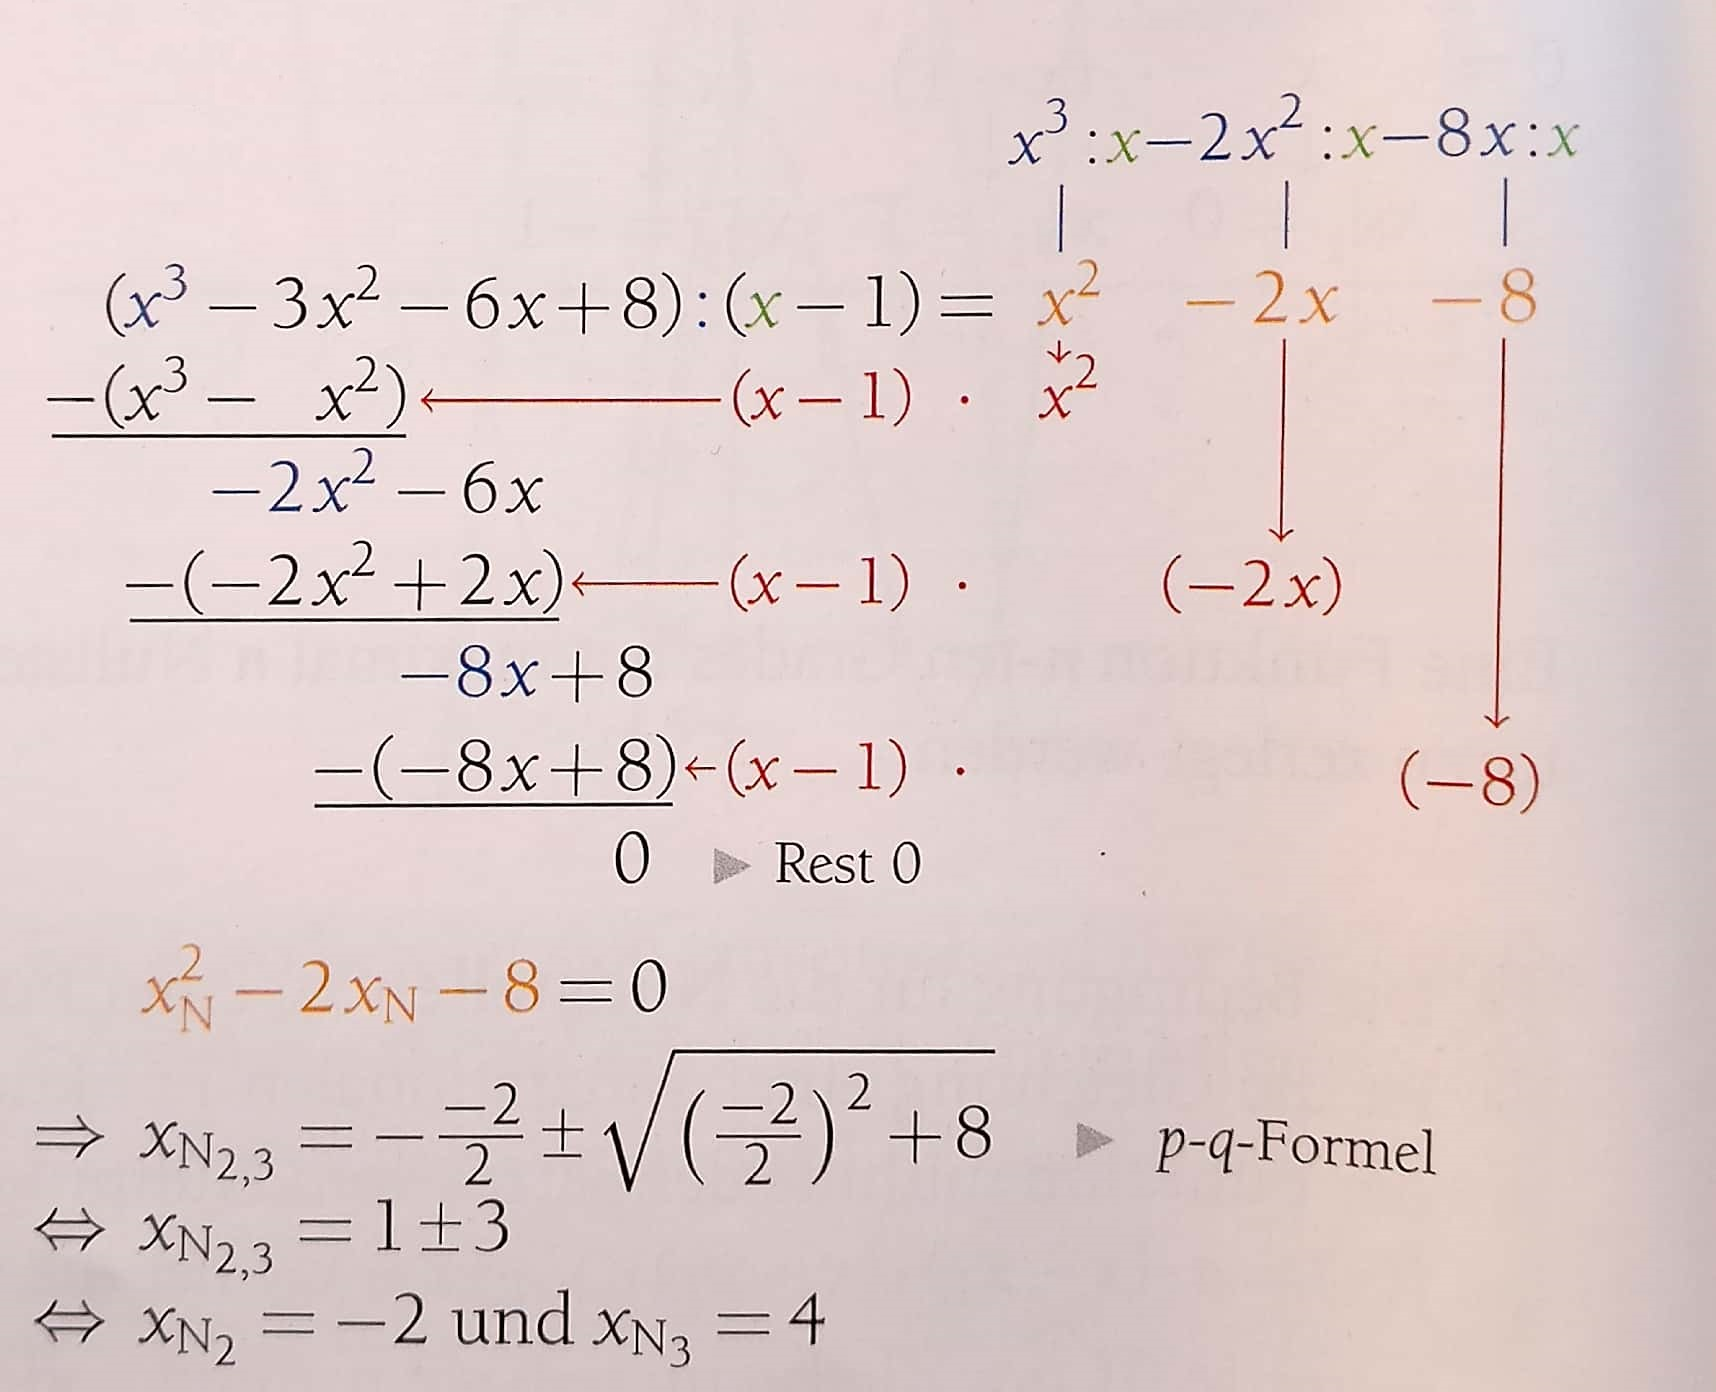
\includegraphics[width=0.48\textwidth]{../99_Bilder/polDiv.jpg}\\
		\tiny{\color{codegray}{\underline{Quelle:} Mathematik Technik\footnote{Schulbuch Mathematik Technik - Fachhochschulreife (Cornelsen)}, S. 116}}\normalsize\\
		\par\noindent
		\underline{\textbf{Ihre Aufgabe:}} Welches wäre das Faktorpolynom, wenn durch \((x-4)\) oder \((x+2)\) geteilt worden wäre?\\
		\par\noindent
		\textit{Bleibt zu klären, wie die einzelnen Summanden des Faktorpolynoms entstehen.} Dazu auf der nächsten Seite mehr.
		\onecolumn
		\subsubsection*{Die Polynomdivision}
		Wir wollen versuchen, das Ganze an einem Beispiel zu verdeutlichen. Gesucht sind die Nullstellen der GRF \(\mathbf{f(x) = x^3+7x^2+2x-40}\). Mit dem Hinweis wissen wir, dass \(\mathit{-40;\ -20;\ -10;\ -8;\ -5;\ -4;\ -2;\ -1;\ 2;\ 4;\ 5;\ 8;\ 10;\ 20}\ \text{und}\ \mathit{40}\) mögliche Nullstellen sind.\\
		Durch einsetzen haben wir \(x=2\) als Nullstelle bestimmt und somit \((x-2)\) als unseren Teiler festgelegt.\\
		Nachfolgend ist die Polynomdivision schrittweise durchgeführt.\\\par\noindent
		Zunächst müssen wir folgendes Problem lösen: \(x\cdot{}\)\fbox{\(?\)} \( = x^3\)?
		\par\noindent
		\begin{tabularx}{0.5\textwidth}{rlllllllllll}
			& \colorbox{green!10}{\(x^3\)} & \(+\)\(7x^2\) & \(+\)\(2x\) & \(-\)\(40\) & \(:\) & (\colorbox{green!10}{\(x\)}\(-\)\(2\)) & \(=\) & \underline{\(x^2\)} & & & \\
			\(-\) & \colorbox{green!10}{\(x^3\)} & \( +\)\(2x^2\) & \multicolumn{1}{c}{|} & & \multicolumn{5}{l}{\color{codegray}{\small{\textit{\(-[x^2(x-2)] = -[x^3-2x^2] = -x^3 - 2x^2\)}}}}\\
			\cline{1-3}
			& & & \multicolumn{1}{c}{\(\downarrow\)}\\
			& & \multicolumn{1}{r}{\(9x^2\)}
		\end{tabularx}
		\par\noindent
		Unser \grq{}Nullstellen-Polynom\grq{} (\(x-2\)) hat zwei Terme. Um also weiter rechnen zu können, müssen wir aus unserem Polynom ein weiteres nach unten ziehen.
		\begin{framed}
			\noindent
			\color{codegray}{\small{\textit{Wieso genau rechnen wir hier Minus?}\\
					Wir haben das Polynom \(\mathbf{f(x) = x^3 +7x^2+2x-40}\) gegeben, teilen dieses durch das \grq{}Nullstellen-Polynom\grq{} \(\mathbf{(x-2)}\).\\
					Es gilt, \((x-2)\) passt \(x^2\)-mal in \(f(x)\). Also ziehen wir \(x^2\cdot{}(x-2)\) von \(f(x)\) ab und schauen dann, wie oft \(x-2\) in den Rest passt.}}
		\end{framed}\normalsize\normalcolor
		\begin{tabularx}{0.5\textwidth}{rlllllllllll}
			& \(x^3\) & \(+\)\(7x^2\) & \(+\)\(2x\) & \(-\)\(40\) & \(:\) & (\colorbox{green!10}{\(x\)}\(-\)\(2\)) & \(=\) & \(x^2\) & \(+\ \)\(9x\)& \\
			\(-\) & \(x^3\) & \( +\)\(2x^2\) & & \multicolumn{1}{c}{|}\\
			\cline{1-3}
			& & \(9x^2\) & \(+\)\( 2x\) & \multicolumn{1}{c}{|}\\
			& & \(-\)\(9x^2\) & \(+18x\) & \multicolumn{1}{c}{|}\\
			\cline{3-4}
			& & & & \multicolumn{1}{c}{\(\downarrow\)}\\
			& & & \multicolumn{1}{r}{\colorbox{green!10}{\(20x\)}} & \\
		\end{tabularx}\\
		\par\noindent
		Auch diesmal brauchen wir wieder den Restterm.\\
		\par\noindent
		\begin{tabularx}{0.5\textwidth}{rlllllll|lll|}
			\cline{9-11}
			& \(x^3\) & \(+\)\(7x^2\) & \(+\)\(2x\) & \(-\)\(40\) & \(:\) & (\colorbox{green!10}{\(x\)}\(-\)\(2\)) & \(=\) & \(x^2\) & \(+\ \)\(9x\)& \(+\ \)\underline{\(20\)}\\
			\cline{9-11}
			\(-\) & \(x^3\) & \( +\)\(2x^2\) & & \multicolumn{1}{c}{|}\\
			\cline{1-3}
			& & \(9x^2\) & \(+\)\( 2x\) & \\
			& & \(-\)\(9x^2\) & \(+18x\) & \\
			\cline{3-4}\\
			& & & \multicolumn{1}{r}{\colorbox{green!10}{\(20x\)}} & \(-\)\(40\) \\
			& & & \(-\)\(20x\) & \(+\)\(40\) \\
			\cline{4-5}
			& & & & \multicolumn{1}{r}{\(0\)}
		\end{tabularx}\\
		\par\noindent
		Wir haben durch Polynomdivison herausgefunden, dass \(\mathbf{x^3+7x^2+2x-40=(x-2)(x^2+9x+20)}\).\\
		Da wir ja die Nullstellen wissen wollten, müssen wir nun nur noch die Nullstellen des zweiten Faktors (\(x^2+9x+20\)) bestimmen. Und wie wir das tun, wissen wir!
%		\polyset{style=C, div=:,vars=x, delims={}{}}
%		\polylongdiv{x^3+7x^2+2x-40}{x-2}\\
	\end{worksheet}
\end{document}